\section{ASR Evolution}

\begin{frame}[allowframebreaks]{ASR Evolution}
Automatic Speech Recognition (ASR) has undergone significant evolution over the past decades. The progression of core technologies is summarized below:

\begin{itemize}
    \item \textbf{GMM-HMM (Gaussian Mixture Model - Hidden Markov Model):}
        \begin{itemize}
            \item Early ASR systems relied on statistical models.
            \item GMMs modeled acoustic features.
            \item HMMs captured temporal dynamics.
            \item \textit{Key paper: Rabiner, 1989.}
        \end{itemize}
    \item \textbf{DNN-HMM (Deep Neural Network - Hidden Markov Model):}
        \begin{itemize}
            \item Deep learning enabled DNNs to replace GMMs for acoustic modeling.
            \item Significant improvement in recognition accuracy.
            \item \textit{Key paper: Hinton et al., 2012.}
        \end{itemize}
    \item \textbf{RNN-HMM (Recurrent Neural Network - Hidden Markov Model):}
        \begin{itemize}
            \item RNNs, especially LSTMs, improved modeling of sequential data.
            \item Better context handling in speech.
            \item \textit{Key paper: Graves et al., 2013.}
        \end{itemize}
    \item \textbf{End-to-End ASR:}
        \begin{itemize}
            \item Modern systems bypass HMMs entirely.
            \item Use architectures such as:
                \begin{itemize}
                    \item Connectionist Temporal Classification (CTC)\\
                    \textit{Graves et al., 2006}
                    \item Attention-based encoder-decoder models\\
                    \textit{Chan et al., 2016 (Listen, Attend and Spell)}
                    \item Transformers\\
                    \textit{Dong et al., 2018}
                \end{itemize}
            \item Direct mapping from audio to text.
        \end{itemize}
\end{itemize}

\framebreak

\begin{figure}
    \centering
    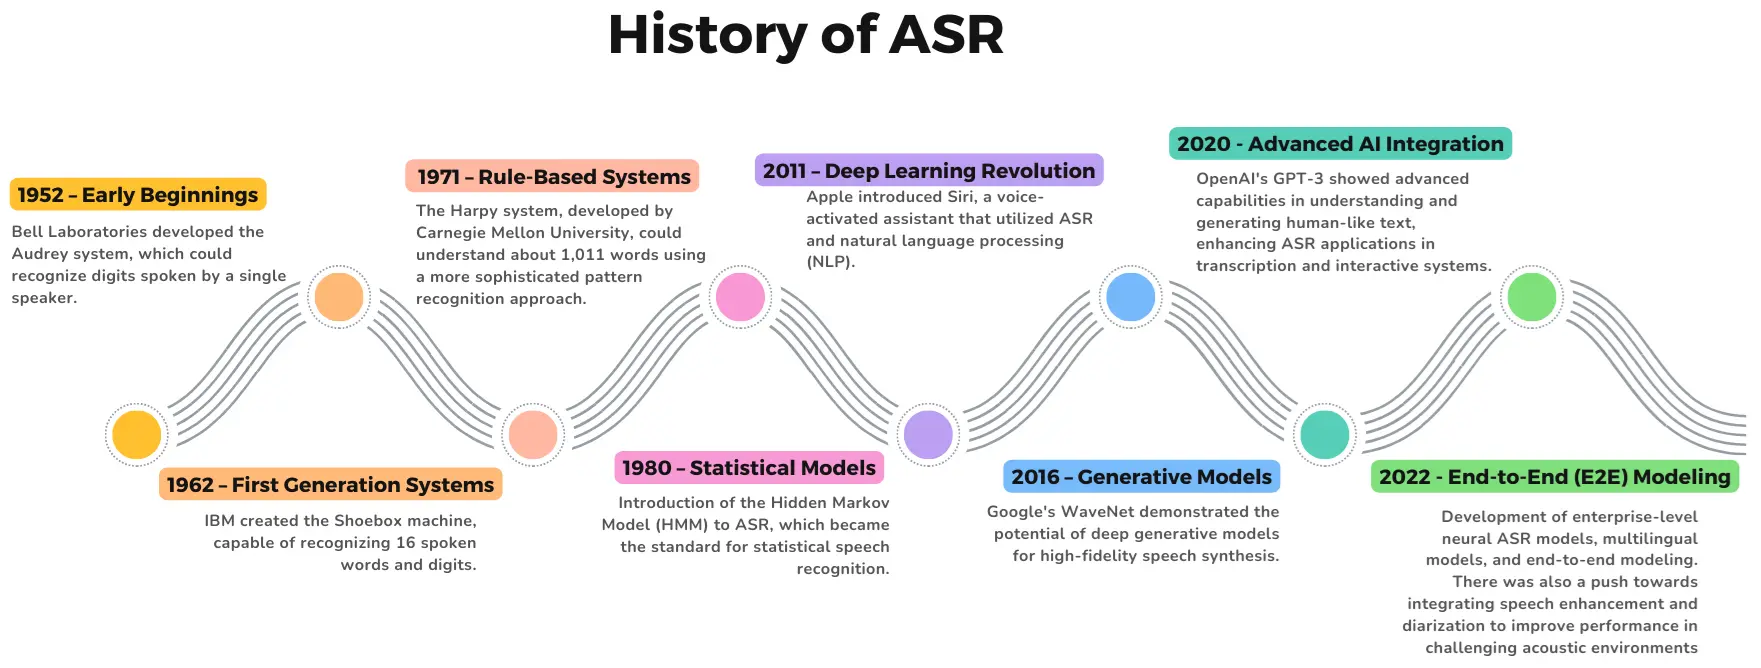
\includegraphics[width=1.08\textwidth,height=0.8\textheight,keepaspectratio]{images/audio-nlp/asr-history.png}
    \caption*{A block diagram for MFCC computation: From audio signal to MFCC features.}
\end{figure}

\framebreak

\textbf{Summary:}
\begin{itemize}
    \item ASR systems have shifted from statistical models to deep learning-based approaches.
    \item Each stage in the evolution brought significant improvements in accuracy and robustness.
    \item End-to-End models simplify the pipeline and enable direct optimization for transcription tasks.
\end{itemize}
\end{frame}